\documentclass[11pt,a4paper]{article}

% ── Packages ──────────────────────────────────────────────────
\usepackage[margin=1in]{geometry}
\usepackage{amsmath,amssymb,amsfonts}
\usepackage{graphicx}
\usepackage{booktabs}
\usepackage{multirow}
\usepackage{caption}
\usepackage{subcaption}
\usepackage[dvipsnames]{xcolor}
\usepackage{hyperref}
\usepackage{cleveref}
\usepackage{enumitem}
\usepackage{microtype}
\usepackage{natbib}
\usepackage{tikz}
\usepackage{pgfplots}
\pgfplotsset{compat=1.18}

\hypersetup{
  colorlinks=true,
  linkcolor=MidnightBlue,
  citecolor=MidnightBlue,
  urlcolor=MidnightBlue
}

% ── Macros ────────────────────────────────────────────────────
\newcommand{\vv}{\mathbf{v}}
\newcommand{\uu}{\mathbf{u}}
\newcommand{\kk}{\mathbf{k}}
\newcommand{\hh}{\mathbf{h}}
\newcommand{\dd}{\mathbf{d}}
\newcommand{\WW}{\mathbf{W}}
\newcommand{\CC}{\mathbf{C}}
\newcommand{\R}{\mathbb{R}}
\newcommand{\E}{\mathbb{E}}
\newcommand{\abs}[1]{\lvert #1 \rvert}
\newcommand{\norm}[1]{\lVert #1 \rVert}
\newcommand{\cosim}{\abs{\cos(\cdot,\cdot)}}

\graphicspath{{../results/figures/}}

% ══════════════════════════════════════════════════════════════
\title{The Dark Subspace: ROME Edits Succeed\\Outside the Model's Linear Concept Geometry}

\author{
  James Elcock
}

\date{}

% ══════════════════════════════════════════════════════════════
\begin{document}
\maketitle
% \institute{The University of Cambridge }

% ──────────────────────────────────────────────────────────────
\begin{abstract}

Modern large language models have increasingly complex architectures and billions to trillions of parameters, all of which makes interpreting such models a highly challenging task. One useful tool is the Linear Representation Hypothesis (LRH) which posits that large language models encode high-level concepts as linear directions in activation space. Other work (ROME) has shown that factual knowledge can be edited to specific pieces of information by altering targeted MLP weights and so changing the residual stream. A natural conjecture then is that this knowledge editing succeeds by changing activations according to these linear concept directions. We conduct eight experiments on GPT-2~XL to test this conjecture systematically and 
we find that (1)~ROME's edit vectors cluster strongly by concept however, they are nearly orthogonal to independently extracted concept directions; (2)~the causal signal lives in a \emph{dark subspace} orthogonal to all identifiable geometric structure, carrying 50--54\% of the edit's efficacy, which reaches 96\% if scaled, while the concept component carries 0\%; and (3)~ that this finding generalises beyond the ROME editing regime, through work using MEND, a different knowledge editing method. We surmise that these knowledge edits \textbf{TO DO ....}

% We conclude that ROME operates through a high-dimensional perturbation that exploits the network's nonlinear dynamics---amplification across layers and attention-mediated broadcasting---rather than the model's linear representational geometry.
\end{abstract}

% ══════════════════════════════════════════════════════════════
\section{Introduction}
\label{sec:intro}
Modern large language models (LLMs) are trained on vast amounts of data and, as a result, encode substantial knowledge in their parameters. It has been shown that LLMs can accurately predict factual statements about the world~\citep{petroni2019language,adelani2021masakhaner,roberts2020much}, and beyond facts, they also encode broader conceptual information~\citep{gurnee2023language,lrhorig}. Understanding the structure of such internal representations and how they interact is a central question in mechanistic interpretability.

The linear representation hypothesis (LRH) is one theory regarding the latent space structure. It proposes that concepts are encoded along linear, near-orthogonal directions in activation space~\citep{mikolov2013linguistic,lrhorig}. Whilst recent work has shown that the strictest version of this hypothesis does not hold in general~\citep{engels2024not} (MORE CITATIONS), mild generalisations, such as treating concept directions as low-dimensional subspaces that allow richer, manifold-like behaviour, combined with strong empirical results showing an underlying linear-like concept structure, allow the core claim to persist~\citep{lrhorig} (MORE CITATIONS).

A separate but related challenge is that of knowledge editing. Once trained, LLMs have no targetted mechanism for updating specific pieces of information stored within. Several knowledge editing approaches have been proposed to address this, such as constrained fine-tuning, meta-learning based editors such as MEND~\citep{mitchell2022fast}, as well as methods such as MEMIT~\citep{meng2022mass} to update many facts simultaneously, at scale.
Among these, Rank-One Model Editing \citep[ROME;][]{meng2022locating} has been shown to be particularly effective for single-fact intervention, achieving a 99.8\% efficacy rate by applying a rank-one update to a targeted MLP weight matrix.

Despite the efficacy of ROME, there has been little work exploring how the learnt edits produced relate to the underlying conceptual structure of the model. For instance, if an edit changes a person's nationality from French to German, does that coincide with the model's existing geometric difference between the concepts of French and German? If such alignment does not hold, then there is the question of what latent space representation is learnt instead in order to make these successful edits? It also raises questions about the potential reliability of the knowledge editing method in practice.

This project aims to bridge these two lines of work by investigating how the vector level, residual stream changes induced by ROME correspond to the concept-level representations described by the LRH. In doing so, we hope to shed light on the mechanism by which ROME is able to edit knowledge as well as the broader geometry of factual knowledge within LLMs.


% Knowledge editing methods modify the factual associations stored in large language models without retraining them.
% Among these, Rank-One Model Editing \citep[ROME;][]{meng2022locating} has become a standard approach, inserting a rank-1 update $\WW' = \WW + \uu \otimes \vv$ into the MLP projection matrix at a single layer.
% ROME achieves high edit success rates while preserving unrelated model behaviour.

% Separately, the Linear Representation Hypothesis \citep[LRH;][]{park2023linear,mikolov2013linguistic} proposes that high-level concepts---nationalities, object categories, relational properties---are encoded as linear directions in activation space.
% Evidence for the LRH comes from linear probing \citep{belinkov2022probing}, mean-difference directions \citep{burns2022discovering}, and causal interventions \citep{geiger2024finding}.

% These two lines of work suggest an appealing hypothesis: \emph{ROME succeeds because its edit vector $\vv$ pushes the model's internal representations along linear concept directions.}
% If the model stores ``LeBron James plays basketball'' as a linear feature, then editing this fact to ``football'' would involve moving the representation along a basketball-to-football direction.
% Under this account, ROME's effectiveness is explained by the LRH: the model's linear concept geometry provides a natural coordinate system for factual editing.

% We test this hypothesis through eight experiments, each addressing a different aspect of the geometric relationship between ROME's edit vectors and the model's concept representations.
% Our findings are uniformly negative: the edit mechanism operates in a subspace orthogonal to every linear geometric structure we can identify.
% This result is robust across extraction methods, edit layers, relation types, and even across a fundamentally different editing algorithm (MEND).

% \paragraph{Contributions.}
% \begin{enumerate}[nosep]
% \item We establish that ROME's $\vv$ vectors are nearly orthogonal to concept directions ($\cosim \approx 0.05$--$0.08$), despite clustering by concept at 97\% LDA accuracy---two parallel but orthogonal linear structures at the same layer.
% \item We identify a \emph{dark subspace}---the component of $\vv$ orthogonal to both concept and clustering directions---that carries the majority of the edit's causal efficacy (50--54\%), while concept and clustering components carry 0\% and 0--10\% respectively.
% \item We show that efficacy and alignment are fundamentally anti-correlated across edit layers ($\rho = -0.72$), with no layer achieving both.
% \item We demonstrate that $\uu$ carries no concept structure (all key-space probes at chance) and edits are $900\times$ entity-selective.
% \item We extend the analysis to MEND and find the same orthogonality, suggesting the finding is structural rather than algorithm-specific.
% \end{enumerate}


% ══════════════════════════════════════════════════════════════
\section{Background}
\label{sec:background}

\subsection{Rank-One Model Editing}

ROME \citep{meng2022locating} treats multi-layer perceptron (MLP) layers as key--value stores, where keys encode subject identity in context and values encode the associated factual knowledge.
The location of a given fact is first identified through \emph{causal tracing}: the network is run multiple times with embeddings systematically corrupted to isolate the layer most responsible for the factual association.
A rank-one update is then applied to the MLP down-projection matrix at a target layer~$\ell$ to overwrite the stored value.

Formally, the MLP computes $\hh = \WW\kk$, where $\WW \in \R^{d_\text{model} \times d_\text{inner}}$ and $\kk \in \R^{d_\text{inner}}$ is the key activation.
The rank-1 update is:
\begin{equation}
  \hat\WW = \WW + \frac{\vv^* - \WW\kk^*}{\kk^{*\top}\CC^{-1}\kk^*} \cdot (\CC^{-1}\kk^*)^\top
  \label{eq:rome}
\end{equation}
where $\kk^*$ is the subject's MLP key, $\CC = \E[\kk\kk^\top]$ is the uncentred second-moment matrix estimated over 100K Wikipedia samples, and $\vv^*$ is the optimised target activation.

This decomposes into two vectors:
\begin{itemize}[nosep]
\item $\uu = \CC^{-1}\kk^* \in \R^{d_\text{inner}}$ : the covariance-whitened subject key, determining when the edit fires.
\item $\vv = (\vv^* - \WW\kk^*) / (\kk^{*\top}\CC^{-1}\kk^*) \in \R^{d_\text{model}}$ : the residual between the optimised target and the current output, determining what changes.
\end{itemize}
This allows us to rewrite the update as
\begin{equation}
    \label{eq:assoc}
    \hat \WW = \WW + \vv \otimes \uu
\end{equation}
with $\vv$ being the residual change and $\uu$ being the new key gating which determines when the change fires. The key $\kk^*$ remains the same as $\kk$ and the target $\vv^*$ is computed via 20 Adam steps (lr\,$=$\,0.5) to maximise $P(\text{target token})$ at the loss layer (layer~47 in GPT-2~XL), with KL-divergence regularisation.
The default edit layer is $\ell = 17$.

\subsection{The Linear Representation Hypothesis}

The LRH states that high-level concepts are encoded as linear directions in activation space \citep{lrhorig}.
Under this hypothesis, there exists a unit vector $\dd \in \R^{d_\text{model}}$ such that $\langle \dd, \hh \rangle$ reveals the degree to which concept $c$ is present in activation $\hh$.

We extract concept directions via two methods:
\begin{itemize}[nosep]
\item \textbf{Mean-difference} \citep{burns2022discovering}: the normalised difference of class centroids for positive (has property) vs.\ negative (lacks property) examples.
\item \textbf{Logistic probing} \citep{belinkov2022probing}: the weight vector of a trained linear classifier, normalised to unit length.
\end{itemize}
% A third method, Distributed Alignment Search \citep[DAS;][]{geiger2024finding}, was evaluated in our pilot study but dropped due to instability in high-dimensional spaces (explained variance $<0.09$).

\subsection{MEND}

Model Editor Networks with Gradient Decomposition (MEND) \citep{mitchell2022fast} provides a natural comparison: it also produces rank-1 updates to MLP projection matrices, but via a learned meta-network rather than per-edit optimisation, and edits layers~45--47 (where concept structure is strong).

% TODO: is this suitable since different layers?

% ══════════════════════════════════════════════════════════════
\section{Experimental Setup}
\label{sec:setup}

All experiments use GPT-2~XL (1.5B parameters, 48 layers, $d_\text{model} = 1600$, $d_\text{inner} = 6400$) with entities drawn from the CounterFact dataset \citep{meng2022locating}, as in the original ROME paper.
We use 10 Wikidata relations spanning several different domains: P176 (manufacturer), P1412 (languages spoken), P37 (official language), P27 (citizenship), P413 (position played), P17 (country), P106 (occupation), P495 (country of origin), P449 (original network), and P937 (work location).
For each relation, we select the top target values and sample entities uniformly within each target.

Residuals and vectors are extracted from layer 17, unless specified. ROME found that this layer is most effective for editing using their regime and so we explore the dynamics at this layer. We also experiment using different probe layers ($[0, 5, 10, 13, 15, 17, 20, 25, 30, 35, 40, 47]$) to explore how the dynamics vary across the model.
Concept directions are extracted using both mean-difference and linear probing to build a logistic classifier (with five fold cross validation), in accordance with (CITATIONS NEEDED)
% Pre-specified thresholds for ``meaningful alignment'' are $\cosim \geq 0.30$ (individual vectors) and $\geq 0.40$ (shared components). NO JUSTIFICATION

\paragraph{Determinism validation.}
ROME computes $\vv$ through gradient optimisation, which could cause problems due to the stochastic nature of this process. We verify that $\vv$ is highly reproducible through repeated runs with fixed context templates, which repeatedly produce identical or near-identical vectors (cosine similarity $= 1.000$ for the same template, $= 0.965$ for different templates).
All subsequent experiments fix templates at the start for reproducibility.


% ══════════════════════════════════════════════════════════════
\section{Findings}
\label{sec:results}

\subsection{Linear Concept Structure Exists In Earlier Layers}
\label{sec:exp1}

Exploring how ROME relates to concepts requires that concepts be encoded as linear directions at layer~17, where ROME injects its edit. Therefore, as an auxiliary result, we need to ensure that concept structure exists in earlier layers, and at least specifically in layer~17. 

\paragraph{Experiment.}
To see whether the concept geometry exists at earlier layers, we calculate the concept vector directions for 10 relations, focussing on the logistic regression produced from linear probing since this can provide accuracy values of a held-out test set, whereas mean difference by nature cannot here. These accuracy scores then allow us to evaluate whether the concepts actually exist in the space.

\begin{figure}[h]
    \centering
    \includegraphics[width=0.8\linewidth]{../results/exp1/probe_accuracy_by_layer.png}
    \caption{\textbf{Concept presence across layers.} We plot the balanced accuracy of linear probes on the concepts found, based on a 30\% held-out test set of counterfactual pairs. The plot shows that concepts are able to be predicted across layers, and whilst the accuracy is better than 50\% chance, the accuracy is not perfect and varies across the concepts themselves. Generally, the balanced accuracy of concept presence prediction increases through the model.}
    \label{fig:prob_acc_layer}
\end{figure}



\paragraph{Results.}
From \Cref{fig:prob_acc_layer}, we can see that broadly, the linear concept structure exists even in earlier layers, with it being highly present for particular concepts (e.g. Japanese-ness). We also find that concept presence is layer-dependent, with concept prevalence increasing for most as the activations propagate further into the model. 
Using the information gained here, for future experiments, we take the top 6 concepts at layer 17, to ensure that the concept vectors we compare to are correct.


\begin{figure}[h!]
    \centering
    \includegraphics[width=0.95\linewidth]{../results/exp1/method_agreement_and_stability.png}
    \caption{\textbf{Concept vectors similarity and consistency.} We plot (a) the cosine similarity between the vectors found by probing and the model produced, (b) the heat map of the cosine similarity between concepts found using mean difference and (c) probing. We see moderate similarity on average across concepts and layers, with some concept vectors (e.g. P27\_Japan) aligning a lot across methods while vectors for other concepts (e.g.P37\_Finnish) are not related.
    }
    \label{fig:method_agreement}
\end{figure}
An additional area of interest is how the concept vectors differ across layers and how the mean difference concept vectors differ from those generated by the logistic model. From \Cref{fig:method_agreement} we can see that the concept vectors found using the mean difference and probing techniques are moderately similar on average. We also see that the concept vectors found by mean difference are more stable and consistent across layers, particularly about the early to middle layers, suggesting these concept vectors are more accurate and robust. %MORE??

Overall these results show that linear concept structure, representative of that described by the LRH exists in earlier layers and in particular in layer 17, allowing for us to fairly compare concept vectors with ROME edit vectors.



% The LRH holds---concepts are linearly decodable---but the geometry is strongest $\sim$23 layers downstream of where ROME operates.
% This creates immediate tension: if concept structure is weak at layer~17, how could ROME be exploiting it there?

% \begin{table}[t]
% \centering
% \caption{Probe balanced accuracy at layer~17 for the 20 binary tasks. Only 6/20 exceed 0.75, peaking at layer~40 where 10/20 pass.}
% \label{tab:probes}
% \small
% \begin{tabular}{@{}lcc@{}}
% \toprule
% Task & Bal.\ Acc.\ (L17) & Pass ($\geq$0.75)? \\
% \midrule
% P27\_Japan    & 0.951 & \checkmark \\
% P37\_Finnish  & 0.849 & \checkmark \\
% P1412\_English & 0.788 & \checkmark \\
% P176\_Honda   & 0.788 & \checkmark \\
% P176\_Toyota  & 0.773 & \checkmark \\
% P937\_London  & 0.759 & \checkmark \\
% P413\_midfielder & 0.741 &  \\
% P1412\_French & 0.741 &  \\
% P17\_India    & 0.700 &  \\
% P37\_English  & 0.673 &  \\
% \addlinespace
% P449\_NBC     & 0.510 &  \\
% \bottomrule
% \end{tabular}
% \end{table}



% ──────────────────────────────────────────────────────────────
\subsection{Edit Vectors Share a Concept Structure That Is Orthogonal to Concept Directions}
\label{sec:exp1b}

With the presence of concept directions in earlier layers established, we can investigate how such concepts relate to ROME edit vectors. If ROME pushes along concept directions, then editing 30~different entities toward the same target (e.g., ``manufactured by Toyota'') should produce $\vv$ vectors that share a common ``Toyota component'' and that component should point along the concept direction described in the concept vectors found.
This directly tests whether ROME edits align with the extracted concept vectors and how much of the edit changes are related to these concepts.

\paragraph{Experiment.}
We conduct 300 ROME edits across 5 relations, each for 2 targets and on 30 entities.
For each concept in which we are performing the edit, we compute $\vv_\text{mean}$ (the average of 30 edit vectors for the concept) and test its alignment with concept directions as computed by mean difference and probing. This allows us to see how similar edit vectors for a given concept are to the concept vector about which they are editing. 

Following from the results, we also evaluate whether edit vectors about a given concept are similar and if they refer to some edit in concept. To do this we substitute the average edit vector for a given concept $\vv_\text{mean}$ in place of the individual $\vv$ vectors (keeping $\uu$ the same for each entity). This allows us to see, through the edit success rate, whether there is some shared conceptual information and structure encoded in the vector and so, whether edit concepts are encoded within a different subspace to the concepts they relate to.

\paragraph{Results.}
Individual edit vectors have very low similarity with the concept they relate to. From the individual similarity columns in Table 1, we see that for both mean difference and probing concept vectors, the cosine similarity with the edit vector is less than 0.125, with the mean for each being 0.066 and 0.063 respectively. This is barely better than a random vector, with its expected cosine similarity being $\sim 0.025$ for $\mathbb{R}^{1600}$.

From the additional investigation, we see that edit vectors do share meaningful structure: the within-concept consistency (cosine of each $\vv_i$ with $\vv_\text{mean}$) ranges from 0.55 to 0.68, with approximately 38\% of each $\vv$'s variance in the shared component.
Critically, we also see that $\vv_\text{mean}$ transfers causally: pairing another entity's $\uu$ with the concept's $\vv_\text{mean}$ achieves 84\% of the original edit efficacy (random~$\vv$: 0\%; wrong-concept~$\vv$: 0\%).

If we then compare this $\vv_\text{mean}$ with the concept directions, we get similar results as with individual edit vectors $\vv_i$, with the mean cosine similarities being 0.107 and 0.098 for each method, showing that these edits relate to a different subspace.

As such we can say that the $\vv$ edit vectors share some concept-specific and causally active structure, but this shared signal is nearly orthogonal to the concept directions identifiable in the model.




\begin{table}[t]
\centering
\small
% \smallskip
\begin{tabular}{l cc cc |c}
\toprule
& \multicolumn{2}{c}{Individual} & \multicolumn{2}{c}{Concept-wise Mean} & \multicolumn{1}{|c}{}\\
\cmidrule(lr){2-3} \cmidrule(lr){4-5}
\textbf{Concept} & Mean Diff. & Logistic & Mean Diff. & Logistic & \textbf{Consistency} \\
\midrule
P176\_Toyota      & .037 & .021 & .044 & .029 & .680 \\
P176\_Honda       & .057 & .023 & .084 & .021 & .669 \\
P1412\_English    & .035 & .020 & .033 & .015 & .597 \\
P1412\_French     & .114 & .088 & .198 & .155 & .574 \\
P37\_English      & .066 & .069 & .116 & .119 & .547 \\
P37\_Finnish      & .065 & .107 & .097 & .175 & .610 \\
P27\_Canada       & .027 & .035 & .010 & .053 & .630 \\
P27\_Japan        & .121 & .110 & .196 & .178 & .627 \\
P413\_midfielder   & .070 & .081 & .113 & .131 & .609 \\
P413\_quarterback    & .112 & .063 & .181 & .103 & .609 \\
\midrule
Median            & .066 & .063 & .105 & .111 & .610 \\
Mean              & .070 & .062 & .107 & .098 & .615 \\
\bottomrule
\end{tabular}
\caption{\textbf{Alignment of ROME edit vectors with concept directions (layer~17)}. \textit{Indiv.}: mean $|\cos(\mathbf{v}_i, \mathbf{d})|$ over 30 edits. \textit{Shared}: $|\cos(\bar{\mathbf{v}}, \mathbf{d})|$. \textit{Consistency}: $\langle\cos(\mathbf{v}_i, \bar{\mathbf{v}})\rangle$. Random baseline $\approx 0.025$. The table shows that concept directions gathered using either mean difference or probing are unrelated to individual edits and the mean across edits for a concept. It also shows that individual edit vector align with the mean for the concept, suggesting a different concept structure is present.
\label{tab:alignment}
}

\end{table}



% ──────────────────────────────────────────────────────────────
\subsection{Edit Vector Geometry: Strong Clustering, Orthogonal to Concept Space}
\label{sec:exp2}

% \begin{table}[t]
% \centering
% \caption{PERMANOVA analysis of 500 $\vv$ vectors. Edit vectors cluster strongly by relation and target value, but this structure is orthogonal to probe-based concept directions (LDA vs.\ concept $\cosim = 0.072$).}
% \label{tab:permanova}
% \small
% \begin{tabular}{@{}lrrr@{}}
% \toprule
% Grouping factor & Pseudo-$F$ & $p$-value & $R^2$ \\
% \midrule
% Target value          & 10.78 & $<$0.0001 & \textbf{0.456} \\
% Relation              & 15.52 & $<$0.0001 & 0.222 \\
% Prompt template       &  9.24 & $<$0.0001 & 0.145 \\
% Entity frequency      &  1.43 & 0.0002   & 0.011 \\
% Random assignment     &  0.90 & 0.944    & 0.016 \\
% \bottomrule
% \end{tabular}
% \end{table}

The previous section examined alignment one concept at a time. We now ask a broader question: across many relations and target values, how do edit vectors organise themselves geometrically? If $\vv$ vectors carry concept information, they should exhibit structure that reflects the identity of the edit. The nature of any structure helps to give insight as to the underlying mechanism behind it. 

\paragraph{Setup.} We compute 500~$\vv$ vectors through ROME edits spanning 10~relations $\times$ 5~targets $\times$ 10~entities. These vectors are then used in three complementary analyses: PERMANOVA (a non-parametric multivariate test for group structure), Linear Discriminant Analysis (LDA), and Linear Relational Embeddings (LREs).

\paragraph{Results.}

\paragraph{Edit vectors have a strong grouped structure.}
PERMANOVA tests whether vectors from the same group (e.g.\ the same target value) are closer together than vectors from different groups, using 10{,}000 random label permutations as a null distribution. This allows us to see whether any such structure exists within relations and entities (and so their underlying concepts).
The results are clear and show that target edit value alone explains 45.6\% of the total variance ($p < 0.0001$) and the underlying relation explains a further 22.2\%, while random grouping yields only $R^2 = 0.016$. As such, in terms of conceptual relation, edit vectors carry a hierarchical imprint of target and relation identity. A nested variance decomposition helps to reinforce this, with relation accounting for 22.2\%, target value within relation for 36.0\%, and entity-level residual for 41.8\%.

\paragraph{This structure has a distinct geometry.}
Now that we know these edit vectors group by concept, we can perform LDA to evaluate the separability and so the inter-group relationship.
Performing LDA to classify $\vv$ vectors by relation achieves \textbf{97\% cross-validated accuracy} (random chance gives $= 10\%$ accuracy ), showing that the concepts are nearly linearly separable along the LDA directions, showing a distinct relation (and so concept) geometry.

Since these edit groups cluster and can be accurately split using LDA, a similar question is raised - do the discriminant directions produced by LDA, that separate edit vectors clusters, coincide with the concept directions from probes? The answer is that they do not with the mean $\cosim$ between LDA axes and probe-derived concept directions being $0.072$, which is effectively orthogonal. 

This helps to further show that the edit vectors are organised by concept but along different axes from those the model uses to represent concepts. 

% Note that this comparison is indirect: concept directions encode entity properties (``is this entity Japanese?'') while LDA directions encode edit-type distinctions (``was this a citizenship edit or a manufacturer edit?''); the alignment test asks whether these two forms of concept-level organisation share geometric structure, and finds they do not.

\paragraph{This geometry is also distinct from LRE embeddings.}
As a final, third independent reference frame, we extract Linear Relational Embeddings \citep[LREs;][]{hernandez2024linearity}. For each relation (e.g.\ ``citizenship''), LREs recover the model's own implicit subject-to-object map: given many (subject, object) pairs, we extract the subject's activation at an early layer and the corresponding object's activation at a later layer, then fit a linear map $\hh_{\text{object}} \approx W\hh_{\text{subject}} + \mathbf{b}$ via ridge regression. The top singular vectors of $W$ capture the principal directions along which the model internally transforms subject representations into object representations for that relation. This is a different geometry that is learned from the model's forward pass, independent of both probes and edit vectors.
The reason for this comparison is that since this method explicitly focusses on subject-object mapping, which is similar to the key-value MLP memory that ROME builds on, the embedding directions produced may align with the ROME edit vectors.

The LRE embeddings perfectly explain the variance across all 10 relations for single layer (16-17)  ($R^2=1.000$) and multilayer edit to output (17-47)  ($R^2=1.000$), showing that this method is able to produce effective embedding directions. 
When we compare these LRE directions with both probe-based concept directions and LDA edit-clustering directions (and also  $\vv_\text{mean}$). The LRE directions align with no other geometry (mean $\cosim < 0.100$ in each case). 

From these collection of results we find that three distinct linear structures thus coexist at layer~17:the model's concept geometry (from probes), the edit-vector geometry (from LDA on $\vv$), and the relational-map geometry (from LREs), with no pair being aligned with any other.

% ──────────────────────────────────────────────────────────────
% \subsection{Layer Propagation: Amplification, Not Rotation}
% \label{sec:exp3}

% \begin{figure}[t]
%   \centering
%   \includegraphics[width=\linewidth]{fig3_layer_propagation.pdf}
%   \caption{\textbf{Left:} The perturbation $\Delta\hh$ is amplified 4--7$\times$ as it propagates from the edit layer (17) to the output (47), with attention broadcasting the signal from the subject token to the last (prediction) token. \textbf{Right:} LDA alignment (edit geometry) decays while concept alignment rises slightly, crossing at layer~30---but both remain below 0.15.}
%   \label{fig:propagation}
% \end{figure}

% \paragraph{Motivation.}
% Experiments~1--2 showed that ROME's edit geometry is orthogonal to concept geometry at layer~17---but concept structure peaks at layer~40.
% A natural rescue hypothesis is that the network's own processing (layers 18--47) \emph{rotates} ROME's signal from its own encoding format into concept-space, analogous to how early layers encode features that later layers decode differently.
% If this rotation occurs, then low alignment at layer~17 is expected: the edit signal is ``encoded'' at the edit site and ``decoded'' into concept-space downstream.
% We test this by tracking the perturbation $\Delta\hh$ at every layer after the edit and measuring whether it progressively aligns with layer-specific concept directions.

% \paragraph{Setup.}
% For 100 ROME edits, we measure $\Delta\hh_\ell = \hh_\ell^{\text{edited}} - \hh_\ell^{\text{original}}$ at every layer, at both the subject token and the last token.
% The rotation hypothesis predicts alignment $\geq 0.40$ by layer~40.

% \paragraph{Result.}
% Alignment rises from 0.057 (layer~17) to 0.093 (layer~35)---real but far below threshold (\Cref{fig:propagation}, right).
% At no layer does the perturbation substantially project onto concept-space.
% Three other phenomena emerge:

% \begin{enumerate}[nosep]
% \item \emph{Amplification.} $\norm{\Delta\hh}$ grows from 80.7 (layer~17) to 345.6 (layer~47, subject) and 541.7 (last token)---a 4--7$\times$ increase (\Cref{fig:propagation}, left).
% \item \emph{Attention-mediated broadcasting.} At layer~17, the edit signal is entirely at the subject token (last-to-subject ratio $= 0.014$). By layer~18, 22\% has moved to the last token. By layer~35, the last token carries \emph{more} perturbation than the subject.
% \item \emph{LDA--concept crossover.} LDA alignment decays from 0.132 to 0.045 while concept alignment rises to 0.093; they cross at layer~30. But both values remain small in absolute terms.
% \end{enumerate}

% A negative correlation between late-layer concept alignment and target probability ($\rho = -0.25$, $p < 0.05$) provides additional evidence that concept alignment is incidental.

% ──────────────────────────────────────────────────────────────
\subsection{The effectiveness of \texorpdfstring{$\vv_\text{mean}$}{v-mean} is mostly due to undetermined residual structure}
\label{sec:exp4}

% \begin{figure}[t]
%   \centering
%   \includegraphics[width=\linewidth]{fig2_causal_decomposition.pdf}
%   \caption{Causal decomposition of $\vv_\text{mean}$. Neither the concept direction ($\sim$1\% of energy) nor the LDA subspace ($\sim$19\%) carries the edit signal. The \emph{residual}---orthogonal to both---achieves 50--54\% efficacy. Full $\vv_\text{mean}$ (74\%) outperforms the residual alone, suggesting a synergistic interaction.}
%   \label{fig:decomposition}
% \end{figure}


Since none of the other geometries tested align with edit vectors, let us focus again on what we know to work. From \Cref{sec:exp1b}, we know that the mean edit for a concept $\vv_\text{mean}$ works causally (84\% efficacy) and that it is orthogonal to concept directions (\Cref{sec:exp1b,sec:exp2}). As such, is there some way to decompose these $\vv_\text{mean}$ vectors to understand which component is responsible for the edit efficacy? This will allow us to understand whether there is some mixture of geometries able to better capture the behaviour or whether it is due to entirely undetermined residual vector geometry.
We focus on two geometric components---the projection onto the concept direction and the projection onto the LDA edit-clustering subspace---and a residual orthogonal to both.
By testing each component as a stand-alone edit (pairing it with the entity's own $\uu$), we can determine whether the causal signal lives in an identifiable geometric structure or in the ``dark'' residual that no probe or discriminant analysis captures.

\paragraph{Setup.}
We decompose $\vv_\text{mean}$ into three orthogonal components and test each as a standalone edit:
\begin{align}
  \vv_\text{concept} &= (\vv_\text{mean} \cdot \hat\dd)\,\hat\dd & &\text{(1\% of energy)} \\
  \vv_\text{LDA}     &= \mathbf{Q}\mathbf{Q}^\top\vv_\text{mean} & &\text{(19\% of energy)} \\
  \vv_\text{dark residual} &= \vv_\text{mean} - \vv_\text{concept} - \vv_\text{LDA} & &\text{(80\% of energy)}
\end{align}
where $\hat\dd$ is the unit concept direction and $\mathbf{Q}$ is the orthogonalised LDA basis.
We tested 550 edits (10 concepts $\times$ 5 entities $\times$ 11 conditions).

\paragraph{Results (\Cref{fig:decomposition}).}

If we take each component ($\vv_\text{concept}$, $\vv_\text{LDA}$, $\vv_\text{residual}$) and renormalise according to the $\vv_\text{mean}$ norm $\norm{\vv_\text{mean}}$, we find that the concept direction is inert, carrying 1\% of the energy and having 0\% efficacy for edits.
We also see that the LDA directions are partially effective, carrying 20\% of the vector energy and having 10\% efficacy. The main component is what remains, which we refer to as the ``dark residual'', accounts for the remaining 80\% of the energy and achieves 54\% efficacy.
From this we can see that whilst the dark residual component is responsible for the majority of the edit result, the LDA discriminant directions are necessary and boost edit performance.
As such, this indicates that although the concept/LDA components contribute little to nothing in isolation, they may stabilise the signal through some form of non-linear processing.
This allows us to see that from $\vv_\text{mean}$, which groups ROME edit vectors by concept, part of the behaviour is able to be described through LDA analysis.

More interestingly, we can explore the efficacy of edits as we vary the scaling. Simply scaling the dark residual component by a factor of three produces edits with 96\% efficacy, which is superior to the edits produced by $\vv_\text{mean}$ (74\% efficacy). We also observe that scaling lower-performing vectors improves their efficacy but not significantly, whereas the dark residual (and $\vv_\text{mean}$) curves show a peak followed by decayed performance as the edit substantially degrades layer performance. It is worth noting that while scaling does improve edit performance, it likely harms model outputs as the scaling grows.



\begin{figure}[t]
  \centering
  \includegraphics[width=\linewidth]{../results/exp4/lda_scaling.png}
  \caption{Causal decomposition of $\vv_\text{mean}$. Neither the concept direction ($\sim$1\% of energy) nor the LDA subspace ($\sim$19\%) carries the edit signal. The \emph{residual}---orthogonal to both---achieves 50--54\% efficacy. Full $\vv_\text{mean}$ (74\%) outperforms the residual alone, suggesting a synergistic interaction.}
  \label{fig:decomposition}
\end{figure}

% \begin{table}[t]
% \centering
% \caption{Efficacy and target probability for each component of $\vv_\text{mean}$, averaged across 10~concepts. ``Rescaled'' conditions match $\norm{\vv_\text{mean}}$, isolating direction from magnitude.}
% \label{tab:decomposition}
% \small
% \begin{tabular}{@{}lcccc@{}}
% \toprule
% Condition & Energy & Efficacy & $P(\text{target})$ \\
% \midrule
% Entity's own $\vv$  & --- & 1.000 & 0.990 \\
% Full $\vv_\text{mean}$  & 100\% & 0.740 & 0.553 \\
% \addlinespace
% Concept (natural) & 1\% & 0.000 & 0.004 \\
% Concept (rescaled) & --- & 0.000 & 0.016 \\
% LDA (natural) & 19\% & 0.000 & 0.009 \\
% LDA (rescaled) & --- & 0.100 & 0.046 \\
% Residual (natural) & 80\% & 0.500 & 0.338 \\
% Residual (rescaled) & --- & 0.540 & 0.410 \\
% \addlinespace
% Concept + LDA & 20\% & 0.000 & 0.011 \\
% Random direction & --- & 0.000 & 0.003 \\
% Wrong concept & --- & 0.000 & 0.003 \\
% \bottomrule
% \end{tabular}
% \end{table}



% ──────────────────────────────────────────────────────────────
% \subsection{Layer Sweep: The Alignment--Efficacy Trade-off}
% \label{sec:exp5}

% % \begin{figure}[t]
% %   \centering
% %   \includegraphics[width=\linewidth]{fig1_layer_sweep.pdf}
% %   \caption{Efficacy--alignment trade-off across edit layers (1,800 edits). As the edit layer moves deeper, concept alignment rises but efficacy falls. No layer achieves both efficacy $\geq 0.60$ and alignment $\geq 0.30$. Layer~17's optimality reflects its position in the factual recall zone, not concept alignment.}
% %   \label{fig:sweep}
% % \end{figure}

% \paragraph{Motivation.}
% All results so far used layer~17, ROME's default.
% But Experiment~1 showed concept structure peaks at layer~40, and Experiment~3 showed the perturbation becomes slightly more concept-aligned as it propagates deeper.
% The obvious escape hatch: maybe the orthogonality is just a layer-17 artefact.
% If we edit at a layer with strong concept structure, $\vv$ might naturally align with concept directions.
% Conversely, if the orthogonality persists across layers, it is a fundamental property of the editing mechanism rather than an accident of layer choice.

% \paragraph{Setup.}
% 1,800 ROME edits across 9 layers $[5, 10, 15, 17, 20, 25, 30, 35, 40]$, with loss layer fixed at~47 throughout (only the edit injection point changes).
% Same entities at every layer for controlled comparison.

% \paragraph{Results (\Cref{fig:sweep}).}
% Spearman correlations reveal the fundamental trade-off:
% \begin{itemize}[nosep]
%   \item Layer depth vs.\ efficacy: $\rho = -0.717$ ($p = 0.030$)
%   \item Layer depth vs.\ alignment: $\rho = +0.817$ ($p = 0.007$)
%   \item Efficacy vs.\ alignment: $\rho = -0.567$ ($p = 0.112$)
% \end{itemize}
% No layer achieves both efficacy $\geq 0.60$ and $\cosim \geq 0.30$.
% The alignment peak ($\cosim = 0.132$ at layer~30) does not coincide with the concept structure peak (probe accuracy $= 0.827$ at layer~40).
% The optimiser compensates at deeper layers with larger perturbations ($\norm{\vv}$ increases 82\% from layer~10 to 40), but magnitude cannot substitute for 30 layers of nonlinear amplification.

% \begin{table}[t]
% \centering
% \caption{Layer sweep summary. Efficacy peaks at layer~17 and declines with depth; alignment increases but saturates below meaningful levels. $\norm{\vv}$ grows as the optimiser compensates for reduced computational leverage.}
% \label{tab:sweep}
% \small
% \begin{tabular}{@{}ccccccc@{}}
% \toprule
% Layer & Efficacy & $\cosim$ (logistic) & Probe Acc. & $\norm{\vv}$ & Consistency & Shared Frac. \\
% \midrule
% 5  & 0.740 & 0.069 & 0.734 & 10.1 & 0.477 & 0.232 \\
% 10 & 0.773 & 0.081 & 0.744 &  7.4 & 0.506 & 0.261 \\
% 15 & 0.793 & 0.099 & 0.737 &  7.6 & 0.583 & 0.347 \\
% \textbf{17} & \textbf{0.810} & \textbf{0.098} & \textbf{0.744} & \textbf{8.1} & \textbf{0.625} & \textbf{0.397} \\
% 20 & 0.792 & 0.084 & 0.744 &  8.5 & 0.676 & 0.463 \\
% 25 & 0.695 & 0.113 & 0.770 &  9.2 & 0.716 & 0.521 \\
% 30 & 0.617 & 0.132 & 0.794 & 10.9 & 0.732 & 0.545 \\
% 35 & 0.380 & 0.114 & 0.817 & 11.9 & 0.746 & 0.577 \\
% 40 & 0.328 & 0.109 & 0.827 & 13.5 & 0.758 & 0.598 \\
% \bottomrule
% \end{tabular}
% \end{table}

% Relations differ dramatically in their depth sensitivity: P27 (citizenship) maintains 55\% efficacy at layer~40, while P413 (position played) drops to 10\%, likely reflecting the depth at which different relation types are processed.

% ──────────────────────────────────────────────────────────────
% \subsection{Gating}
% \label{sec:exp67}

% \begin{figure}[t]
%   \centering
%   \includegraphics[width=\linewidth]{fig5_uv_clustering.pdf}
%   \caption{Comparison of concept structure in $\vv$-space (payload) vs.\ $\uu$-space (gate). The payload carries strong concept clustering (8$\times$ higher PERMANOVA $R^2$, 3$\times$ higher LDA accuracy); the gate carries almost none.}
%   \label{fig:uv}
% \end{figure}

% \paragraph{Motivation.}
% Experiments~1--5 analysed $\vv$, the payload.
% But ROME's full edit effect is $(\uu \cdot \kk) \times \vv$: the gate vector $\uu$ determines \emph{when} the edit fires by computing a dot product with the MLP key of each input.
% Even if $\vv$ is concept-orthogonal, concept structure in $\uu$ could make the edit concept-selective---firing not just for the edited entity but for all entities sharing that concept.
% We test this possibility by analysing $\uu$'s geometry, probing the MLP key space for concept information, profiling the gate activation across entities, and finally measuring the full functional consequence: does the assembled edit $\WW + \uu \otimes \vv$ actually change outputs for same-concept entities?

% \paragraph{$\uu$-space geometry.}
% 500 $\uu$ vectors show minimal concept structure (\Cref{fig:uv}): PERMANOVA $R^2 = 0.027$ by relation (vs.\ 0.222 for $\vv$); LDA accuracy $= 0.340$ (barely above chance of 0.10).

% \paragraph{Key-space probes.}
% Every single probe across all 50 tasks (10 relations $\times$ 5 targets) achieves exactly chance accuracy (0.50).
% Concept identity is completely undecodable from MLP key activations at layer~17.

% \paragraph{Gate activation profiling.}
% The gate fires $38\times$ stronger for the edited entity than for same-concept entities (mean activation 10.1 vs.\ 0.26).
% The apparent d$' = 0.46$ for concept selectivity is almost entirely a prompt template artefact: after controlling for template structure within each relation, d$' = 0.017$.

% \begin{figure}[t]
%   \centering
%   \includegraphics[width=\linewidth]{fig4_edit_specificity.pdf}
%   \caption{Edit specificity: ROME edits are $900\times$ more selective for the edited entity ($\Delta P = 0.98$) than for same-concept entities ($\Delta P = 0.002$). The KL hierarchy confirms zero concept-level generalisation.}
%   \label{fig:specificity}
% \end{figure}

% \paragraph{Functional specificity test.}
% The geometric analysis above examines components in isolation.
% We now test the assembled edit: when you apply $\WW' = \WW + \uu\otimes\vv$, does it change outputs for entities other than the target?
% For 50 ROME edits, we evaluate on 4 conditions $\times$ 20 test entities: self, same-target, same-relation, and different-relation (3,050 total evaluations).

% The edit is $\sim$\,$900\times$ more selective for the target entity than for any other (\Cref{fig:specificity}, \Cref{tab:specificity}).
% All 50 self-edits succeeded ($\Delta P > 0.5$); zero non-self edits showed meaningful $\Delta P$.
% The KL divergence hierarchy---self (8.0) $\gg$ same-target (0.009) $\gg$ same-relation (0.004) $\gg$ different-relation (0.0002)---confirms that the edit is surgically entity-specific with no concept-level generalisation.

% \begin{table}[t]
% \centering
% \caption{Edit specificity across conditions. The KL hierarchy confirms surgical entity-level targeting.}
% \label{tab:specificity}
% \small
% \begin{tabular}{@{}lcrc@{}}
% \toprule
% Condition & $\Delta P(\text{target})$ & KL divergence & $n$ \\
% \midrule
% Self (edited entity)    & 0.980  & 8.004  & 50 \\
% Same target value       & 0.002  & 0.009  & 1{,}000 \\
% Same relation           & 0.002  & 0.004  & 1{,}000 \\
% Different relation      & 0.00001 & 0.0002 & 1{,}000 \\
% \bottomrule
% \end{tabular}
% \end{table}

% ──────────────────────────────────────────────────────────────
\subsection{Cross-Method Generalisation: MEND}
\label{sec:exp8}


% TO DO!!!

% \begin{figure}[t]
%   \centering
%   \includegraphics[width=\linewidth]{fig7_rome_vs_mend.pdf}
%   \caption{ROME (layer~17) vs.\ MEND (layer~47). Both methods show low concept alignment ($< 0.15$), despite MEND editing at layers with strong concept structure. ROME's $\vv$ vectors cluster more tightly (LDA~0.97 vs.~0.75).}
%   \label{fig:mend}
% \end{figure}

One final question to ask is whether the orthogonality is specific to ROME or structural to model editing itself.
ROME computes $\vv$ via per-edit gradient optimisation with KL regularisation, and so perhaps the optimiser specifically avoids concept-aligned directions to minimise collateral damage.
We compared against MEND \citep{mitchell2022fast} since it also produces rank-1 updates to MLP projection matrices, but via a learned meta-network (a single forward pass) rather than per-edit optimisation, and it edits layers~45--47 where concept structure is strong (\Cref{sec:exp1}).
If MEND's $\vv$ vectors also avoid concept directions, the orthogonality is a property of successful editing itself, not ROME's optimisation landscape.

\paragraph{Setup.}
We perform 200 MEND edits. We extract $\vv$ vectors via SVD of weight deltas (exact for rank-1 matrices; we report layer~47 where the delta is reliably rank-1, fraction $\geq 0.99$).

\paragraph{Results.}
MEND's concept alignment at layer~47: mean-diff $\cosim = 0.121$, logistic $\cosim = 0.068$.
Wrong-concept alignment is nearly as high (0.094), meaning whatever small alignment exists is not concept-specific.
MEND's $\vv$ vectors cluster less than ROME's (LDA~0.75 vs.~0.97; PERMANOVA $R^2 = 0.179$ vs.\ 0.456).

Two methods, two mechanisms, two layer ranges---same result: \textbf{successful edits avoid concept-aligned subspaces.}


% ══════════════════════════════════════════════════════════════
\section{Discussion}
\label{sec:discussion}

\subsection{Two Parallel Linear Structures}

Our central finding is that two well-organised linear concept structures coexist at the same layer but are geometrically orthogonal (\Cref{fig:schematic}):

\begin{enumerate}[nosep]
\item \textbf{Representational geometry}: the directions along which linear probes decode concepts from activations. Strongest at layers~35--40.
\item \textbf{Edit geometry}: the directions along which ROME's $\vv$ vectors organise by concept. Strong at layer~17 (97\% LDA accuracy).
\end{enumerate}

These structures share only $\sim$5--8\% cosine overlap.
The model's concept language and ROME's edit language are nearly independent coordinate systems in the same high-dimensional space.

\begin{figure}[t]
\centering
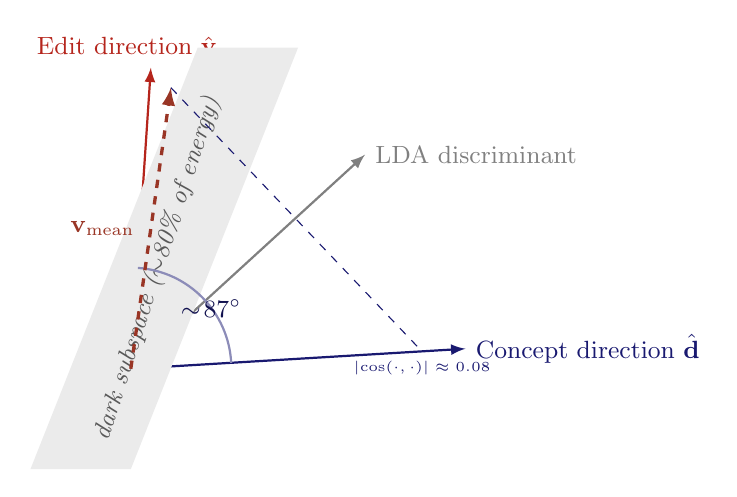
\begin{tikzpicture}[>=latex, scale=0.85, every node/.style={font=\small}]
  % Coordinate axes
  \draw[->, thick, MidnightBlue] (0,0) -- (5,0.3) node[right] {Concept direction $\hat{\dd}$};
  \draw[->, thick, BrickRed] (0,0) -- (0.3,4.5) node[above] {Edit direction $\hat{\vv}_\text{mean}$};
  \draw[->, thick, Gray] (0,0) -- (3.5,3.2) node[right] {LDA discriminant};

  % The dark subspace
  \fill[black!8] (-1.5,-1.5) -- (1.0, 4.8) -- (2.5, 4.8) -- (0.0, -1.5) -- cycle;
  \node[rotate=72, Gray!70!black] at (0.4, 1.5) {\textit{dark subspace ($\sim$80\% of energy)}};

  % Angle arc
  \draw[MidnightBlue!50, thick] (1.5,0.09) arc[start angle=3, end angle=86, radius=1.5];
  \node[MidnightBlue!70!black] at (1.2, 0.9) {$\sim\!87^\circ$};

  % v_mean arrow
  \draw[->, very thick, BrickRed!80!black, dashed] (0,0) -- (0.6, 4.2)
    node[midway, left=2pt] {$\vv_\text{mean}$};

  % Small projections
  \draw[MidnightBlue, dashed, thin] (0.6, 4.2) -- (4.35, 0.261);
  \node[MidnightBlue, below] at (4.35, 0.261) {\tiny $\cosim \approx 0.08$};
\end{tikzpicture}
\caption{Schematic of the geometric relationship at layer~17. The edit direction ($\vv_\text{mean}$) is nearly orthogonal ($\sim$87$^\circ$) to the concept direction ($\hat\dd$). The vast majority of the edit's energy and causal efficacy resides in the dark subspace, orthogonal to both identified structures.}
\label{fig:schematic}
\end{figure}


\subsection{The Dark Subspace}

The causal decomposition (\Cref{sec:exp4}) reveals that the mechanism lives in neither identified structure.
The concept component (1\% of energy) achieves 0\% efficacy; the LDA component (19\%) achieves 0--10\%; the residual (80\%) achieves 50--54\%.

The interpretation is natural: the optimisation target for $\vv^*$ is \emph{behavioural}---maximise $P(\text{target token})$ at layer~47 while minimising KL divergence.
This objective does not reference internal concept geometry; it references only the output distribution.
In $\R^{1600}$ there are vastly more dimensions orthogonal to any $k$-dimensional concept subspace than within it, so the optimiser's solution space is overwhelmingly dark.

% \subsection{The Mechanism: Perturbation, Not Semantic Rewriting}
% NOTE: This subsection references the layer propagation experiment (sec:exp3) which is currently commented out.
% Uncomment if that experiment is restored, or remove entirely.

% The layer propagation analysis (\Cref{sec:exp3}) reveals the actual mechanism.
% Rather than rotating the representation along a concept direction, ROME injects a perturbation at layer~17 that is:
% \begin{enumerate}[nosep]
%   \item \emph{Amplified} 4--7$\times$ through subsequent layers
%   \item \emph{Broadcast} from the subject token to the prediction position via attention (22\% by layer~18, $>$100\% by layer~35)
%   \item \emph{Concentrated at the prediction site} in a way that shifts the relevant logits
% \end{enumerate}
% This is a computational mechanism (exploiting the network's dynamics) rather than a representational one (pushing along concept directions).
% Layer~17's optimality reflects its position in the ``factual recall zone'' \citep{meng2022locating} where the network's processing dynamics provide maximum leverage for converting a compact perturbation into a targeted logit shift.

\subsection{Implications}

\paragraph{For interpretability.}
The LRH correctly describes how concepts are represented, but this representational geometry does not relate to how the model can be edited. We see that two well-organised linear structures can coexist at the same layer without interacting, suggesting that the residual stream's high dimensionality supports multiple independent functional subspaces and so a potential, separate LRH for knowledge editing.

\paragraph{For model editing.}
Editing methods succeed through a mechanism opaque from the perspective of probed linear concept geometry, but instead in their own edit linear concept geometry. As such, methods designed to explicitly operate along concept directions (e.g., steering vectors) act in a fundamentally different setting and are solving a different problem than knowledge editing. This also explains why ROME edits are phrasing-specific (`` `The iconic landmark in Seattle
is the Space Needle' is stored separately from `The Space Needle is the iconic landmark in Seattle' ''~\citep{meng2022locating}) rather than generalising as the mechanism doesn't engage broader, concept-level representations.


\subsection{Limitations}

\begin{enumerate}[nosep]
\item \textbf{Model scope.} All experiments use GPT-2~XL (1.5B). Larger models may exhibit different geometry.
\item \textbf{Direction extraction.} We use mean-difference and logistic probing in Euclidean space. Other probing methods may be able to capture the behaviour of edit vectors.
\item \textbf{Computational constraints.} To explore the effect of edits, we use samples of hundreds of edits across a subset of 10 relations. A more thorough analysis would ideally use on the order of thousands or tens of thousands across hundreds or more relations, to ensure such behaviour is consistent.


% \item \textbf{MEND rank structure.} MEND's weight deltas at layers~45 and 46 are not strictly rank-1 (fractions $\sim$0.72 and $\sim$0.42). Our SVD extraction is approximate there; layer~47 ($\geq$0.99) is the reliable comparison.

% \item \textbf{Concept coverage.} Our 10 relations cover factual/relational knowledge. Sentiment, syntactic features, or world knowledge may interact differently with editing. INCULDE MORE???
\end{enumerate}


% ══════════════════════════════════════════════════════════════
\section{Related Work}
\label{sec:related}

\citet{meng2022locating} introduced ROME and causal tracing, identifying layers~15--20 as the factual recall zone.
\citet{geva2021transformer} characterised MLP layers as key--value memories.
\citet{hernandez2024linearity} extracted Linear Relational Embeddings that map subjects to objects via low-rank linear transformations.
\citet{marks2024geometry} studied the geometry of truth representations.
\citet{hase2024does} identified an inconsistency in ROME's implementation; we replicate and verify our findings under their fix (r-ROME) in the Appendix (\Cref{app:rrome}).
\citet{decao2021editing} and \citet{mitchell2022fast} proposed alternative editing approaches.
Our work is distinguished by its systematic geometric analysis connecting editing mechanisms to representational structure.


% ══════════════════════════════════════════════════════════════
\section{Conclusion}
\label{sec:conclusion}

We systematically tested whether ROME's editing mechanism operates along the linear concept geometry predicted by the LRH.
Experiments provide convergent evidence for a negative answer:
ROME's edit vectors are nearly orthogonal to concept directions ($\cosim < 0.08$),
the causal signal lives in a dark subspace that is unidentifiable yet has a linear concept structure and this same orthogonality holds for other knowledge editing regimes (MEND).
%MORE



% ROME succeeds not by rewriting the model's concept representations, but by injecting a high-dimensional perturbation that exploits the network's nonlinear dynamics---amplification through layers and attention-mediated broadcasting---to shift output logits.
Overall we can conclude that the LRH describes how concepts are represented but it does not play any role in how information is edited, which instead has its own linear geometry.

% ══════════════════════════════════════════════════════════════
\bibliographystyle{plainnat}
\bibliography{references}

% ══════════════════════════════════════════════════════════════
\appendix

\section{r-ROME Sensitivity Analysis}
\label{app:rrome}

\citet{hase2024does} identified an inconsistency in ROME's \texttt{compute\_v} whereby the final rescaling step uses only the final prompt (not all context templates) to estimate current input/output, while \texttt{compute\_u} averages across all context templates.
The fix (``r-ROME'') averages across templates in both functions so that it matches the proper mathematical definition (as in Section 2.1). We reimplemented this fix and reran Experiments~1--4.

\begin{table}[h]
\centering
\caption{r-ROME replication. All direction-based findings replicate within $\pm$0.02.}
\label{tab:rrome}
\small
\begin{tabular}{@{}lrrr@{}}
\toprule
Metric & ROME & r-ROME & $\Delta$ \\
\midrule
\multicolumn{4}{@{}l}{\emph{Experiment 1}} \\
Median $\cosim$ (shared) & 0.111 & 0.112 & $+$0.001 \\
Mean shared fraction & 0.385 & 0.383 & $-$0.002 \\
Shared-$\vv$ transfer efficacy & 0.380 & 0.333 & $-$0.047 \\
\addlinespace
\multicolumn{4}{@{}l}{\emph{Experiment 2}} \\
PERMANOVA $R^2$ (target) & 0.456 & 0.452 & $-$0.004 \\
LDA CV accuracy & 0.970 & 0.968 & $-$0.002 \\
$\cosim$ (concept, $\vv_\text{mean}$) & 0.047 & 0.049 & $+$0.002 \\
\addlinespace
\multicolumn{4}{@{}l}{\emph{Experiment 3}} \\
Peak concept alignment (L35) & 0.093 & 0.093 & 0.000 \\
$\rho$(alignment, target prob) & $-$0.251 & $-$0.300 & $-$0.049 \\
\addlinespace
\multicolumn{4}{@{}l}{\emph{Experiment 4}} \\
Residual efficacy (natural) & 0.500 & 0.520 & $+$0.020 \\
Concept efficacy (any scale) & 0.000 & 0.000 & 0.000 \\
\bottomrule
\end{tabular}
\end{table}

The r-ROME fix changes $\vv$ magnitudes but not directions and since all LRH analyses are direction-based, results are nearly identical.





\end{document}
